\chapter{GROMACS Tutorial: Self-Assembly of lipid bilayer with MARTINI FF}

MARTINI is a coarse-grained force field. In this tutorial, we simulate the self assembly of a lipidic bilayer membrane
in a water environment. 


\begin{figure}[H]
    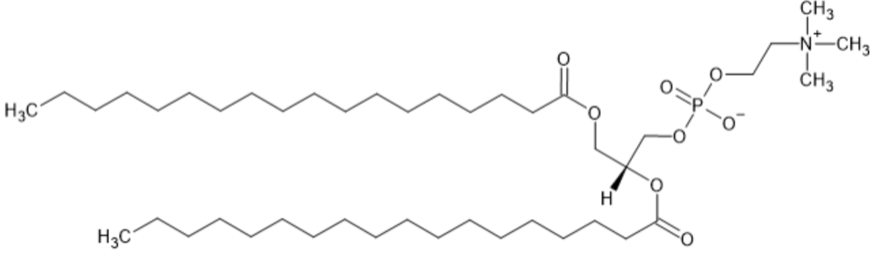
\includegraphics[width=\textwidth]{practicals_img/gromacs/dspc_molecule.png}
    \caption{Di - Stearoyl - Phosphatidyl - Choline: It is a phospholipid, a natural constituent of cellular membranes.
    It features two stearic chains, and its head has both a phosphate group ($PO_4$) and a coline group ($N (CH_3)_4$).}
\end{figure}


The folder contains a lot of files. Let's navigate through them and understand what each contains.
There are basically $5$ extensions that you need to learn:

\begin{itemize}
    \item \textbf{.gro}: GROMACS structure files. Such files contain atomic or coarse-grained coordinates (positions, sometimes velocities)
    of your molecule.
    \item \textbf{.mdp}: stands for \textbf{M}olecular \textbf{D}ynamics \textbf{P}arameter file. These files contain simulation settings. For instance, \textbf{martini3.mdp} contains
    integrator type, timestep, temperature and pressure couplings, cutoffs. And \textbf{minimization.mdp} contains the settings for the energy minimization (method, number of steps). Files with 
    extension .mdp are passed as argument to gromacs command \textbf{grompp}.
    \item  \textbf{.itp/.top}: stands for \textbf{I}nclude \textbf{T}o\textbf{p}ology.  These files contain the actual force field definition, including all its parameters (bead types, bonded interactions terms, unbonded interactions).
    \item \textbf{.tpr}: while the preceeding files are text, this is instead a binary file, so it is not human readeable. It is generated by the gromacs command \textbf{grompp} and bundles everything GROMACS need to run a simulation,
    putting together information about topology, settings and structure. After creating the .tpr file, we can finally run the simulation with the gromacs command \textbf{mdrun}.
    \item \textbf{.trr, .tng, xtc}: trajectory files.
\end{itemize}


\paragraph{Content of the provided files}

\begin{enumerate}
\item dspc\_single.gro, water.gro: configuration of a single molecule of DSPC and a single molecule of water, respectively;
\item martini3.mdp: settings for the use of the martini ff. These include integrator type, timestep, temperature and pressure couplings, cutoffs.
\item minimization.mdp: settings for the minimization step. These include minimization method and number of steps.
\item martini\_v3.0.0.itp: the file defining the core of the MARTINI force field.
\item martini\_v3.0.0\_phospholipids\_v1.itp: specifies how MARTINI represents phospholipids (in terms of coarse grained beads) and the force parameters.
\item martini\_v3.0.0\_solvents\_v1.itp: specifies how MARTINI represents and treats solvents.
\end{enumerate}